\section{Sobre formas alternativas de definición de la base $\cali{L}^{n}$}

Fijada una dimensión $n$,
vamos a generalizar los tipos de objetos
usados
en el método por medio del cual
se definió a la base de Legendre discreta $\cali{L}^{n}$
(en la subsección 
\ref{Generalización que involucra a la discretización Omega n}),
y además, como prometimos en la introducción,
vamos a dar una segunda forma natural
de abordar el problema, cambiando el método de 
discretización
(en la subsección 
\ref{Construcción de Ln en base a discretizaciones con sumas integrales}),
llegando, como se anticipó, a la base
$\cali{L}^{n}$.

\subsection{Construcción generalizada de los PDL usando la discretización $\Omega_{n}$}
\label{Generalización que involucra a la discretización Omega n}

Recuerde que, al definir a los espacios
de polinomios discretos
$W_{n,i}$ en \eqref{def de espacios Wk},
consideramos a
las funciones polinomiales 
$f_{k}(t)=t^{k}$, con $0 \leq k \leq n-1$, que después
discretizamos en la malla uniforme
$\cali{P}_{n}= \{ j: \hspace{0.1cm} 0 \leq j \leq n-1 \} $
para obtener los vectores $v_{k}$; nos
disponemos a probar que, si hubiésemos escogido
\begin{itemize}
\item funciones polinomiales
\[
g_{k}(t) \in \IR[t], \hspace{1cm} 
\text{con }\hspace{0.5cm} 0 \leq k \leq n-1 \hspace{0.2cm} \text{entero},
\]
donde
el grado de $g_{k}$ es $k$ y su coeficiente principal 
$c_{k}$ es positivo, y

\item cualquier malla uniforme de $n$ puntos
\[
\cali{P}=\{t_{j} : \hspace{0.1cm} 0 \leq j \leq n-1 \},
\]
\end{itemize}
si 
\begin{equation}
\label{eq1: 31Oct}
w_{k} := \Omega_{n,\cali{P}}(g_{k})
=(g_{k}(t_{j}))_{j=0}^{n-1}, \hspace{0.3cm} 0 \leq k \leq n-1,
\end{equation}
entonces estos vectores $w_{k}$
generan a los mismos espacios $W_{n,i}$
de antes y,
después de ortonormalizar con el 
método de Gram-Schmidt
al subconjunto $\{w_{k}: \hspace{0.2cm} 0 \leq k \leq n-1\}$
de $\IR^{n}$, obtendríamos la 
base de Legendre discreta $\cali{L}^{n}$ 
definida en \eqref{eq: base de Legendre discreta}. 


\begin{ejemplo}
Sea $n=3$; sean las colecciones de polinomios
\begin{equation}
\label{eq11: 10Dic}
\{
f_{0}(t), 
f_{1}(t), f_{2}(t) \},
\end{equation}
con los polinomios $f_{k}$ como se definieron en \eqref{fk}, y
\begin{equation}
\label{eq12: 10Dic}
\left\{
g_{0}(t):=3,  
g_{1}(t):=\frac{1}{2}t+1,
g_{2}(t):=t^{2}+2t+3 \right\}.
\end{equation}

Las colecciones \eqref{eq11: 10Dic} y \eqref{eq12: 10Dic}
tienen en común que contienen, por cada $0 \leq k \leq 2$,
un polinomio de grado $k$ y coeficiente principal positivo.
Sean $\cali{P}_{3}$ la malla dada por 
\eqref{malla Pn} con $n=3$, o sea, sea 
$\cali{P}_{3}=\{0, 1, 2 \}$, y sea $\cali{P}:= \{
-2, -\frac{1}{2}, 1 \}$ otra malla uniforme de tres puntos.


\begin{figure}[H]
	\sidecaption{
	Ejemplo concreto del proceso tomando 
		las dos colecciones
    de polinomios \eqref{eq11: 10Dic} y \eqref{eq12: 10Dic}, 
    discretizándolas, respectivamente, en las mallas uniformes 
    $\cali{P}_{3}$ y $\cali{P} =\{-2, -\frac{1}{2}, 1 \}$.
	\label{fig: generalizacion def basada en discr puntual}
	} 
	\centering
	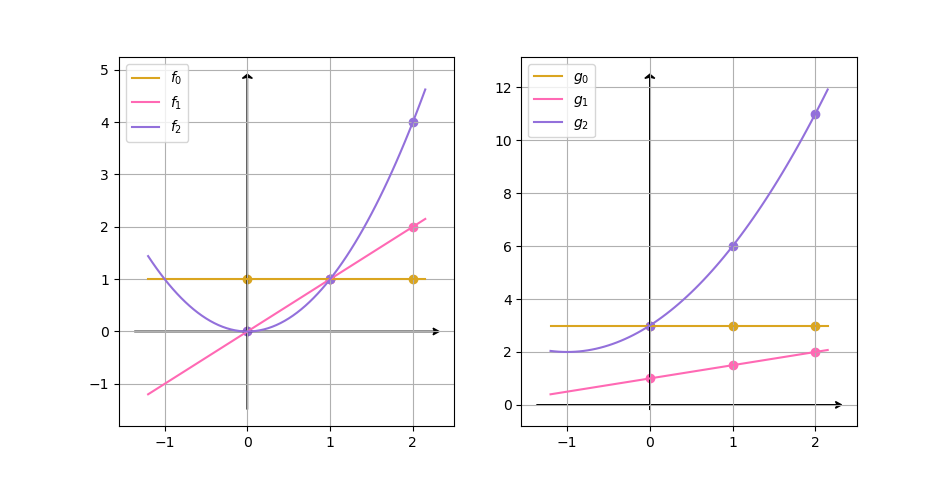
\includegraphics[scale=0.25]{EsquemaGral} 
\end{figure}	

Afirmamos que, si
\begin{itemize}
\item \textcolor{ameMorado}{{(Discretización)}}
consideramos, para $0 \leq k \leq 2$, a los vectores
\[
v_{k}:= \Om_{3, \cali{P}_{3}}(f_{k})
\hspace{0.2cm} \text{y} \hspace{0.2cm}
w_{k}:= \Om_{3, \cali{P}}(g_{k}),
\]
\item \textcolor{ameMorado}{{(Ortogonalización)}}
en base a estos definimos a los vectores
$$ \bar{\xi}_{0}:= v_{0}, 
\hspace{0.2cm} \bar{\eta}_{0}:= w_{0}, 
$$
$$ \bar{\xi}_{k}:= v_{k} - \Pi_{W_{k-1}}(v_{k}), \hspace{0.2cm}
\bar{\eta}_{k}:= w_{k} - \Pi_{W_{k-1}}(w_{k})
\hspace{0.2cm} \text{para} 
\hspace{0.1cm}
k=1,2, $$ y, finalmente, 
\item \textcolor{ameMorado}{{(Normalización)}}
definimos, para toda $0 \leq k \leq 2$,
a los vectores
$$\xi_{k}:= \frac{\bar{\xi}_{k}}{|| \bar{\xi}_{k} ||},
\hspace{0.2cm}
\eta_{k}:= \frac{\bar{\eta}_{k}}{|| \bar{\eta}_{k} ||},
$$
\end{itemize}
entonces, ocurre que
\[
\forall \hspace{0.1cm} 0 \leq k \leq 2:
\hspace{0.2cm} \xi_{k}= \eta_{k}.
\]
\final
\end{ejemplo}

%\begin{tcolorbox}[title=Ejemplo]

%	\begin{figure}[H]
%	\centering
%	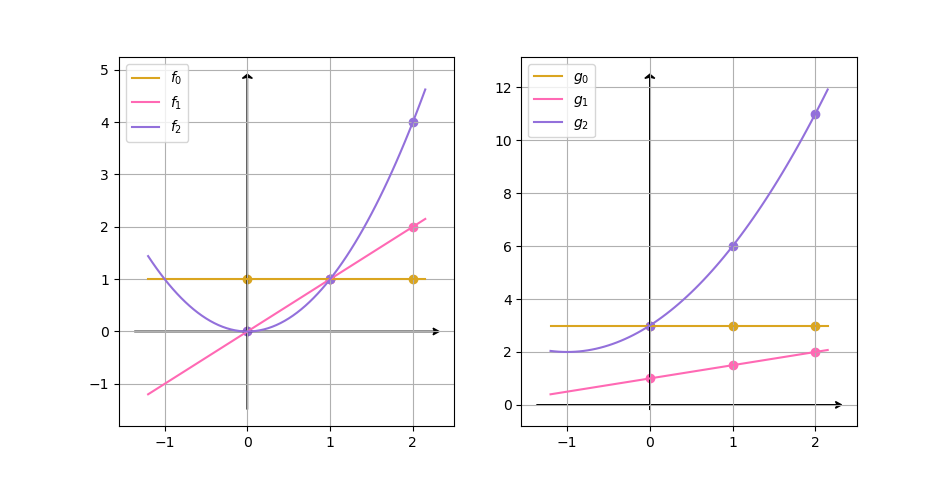
\includegraphics[scale=0.45]{EsquemaGral}
%	\caption{Ejemplo concreto del proceso tomando dos colecciones
 %   de polinomios (a saber, $f_{0}$,  $f_{1}$, $f_{2}$,
  %  y $g_{0}(t):=3$, $g_{1}(t):=\frac{1}{2}t+1$, $g_{2}(t):=t^{2}+2t+3$)
 %   discretizándolas, respectivamente, en las mallas uniformes 
 %   $\cali{P}_{3}$ y $\cali{P} =\{-2, -\frac{1}{2}, 1 \}$.}
%	\end{figure}	

%\tcblower
%\begin{center}
%1.- Discretización
%\end{center}
%\begin{tcbitemize}[raster equal height,colframe=white,colback=white,
%raster every box/.style={minimum for current equal height group=2cm}]
%\tcbitem Consideramos a los vectores
%$$v_{k}:= \Om_{3, \cali{P}_{3}}(f_{k}),$$ con
%$k=0,1,2$.
%\tcbitem Consideramos a los vectores
%$$w_{k}:= \Om_{3, \cali{P}}(g_{k}),$$ con
%$k=0,1,2$.
%\end{tcbitemize}

%\DrawLine

%\begin{center}
%2.- Gram-Schmidt
%\end{center}
%\begin{tcbitemize}[raster equal height,colframe=white,colback=white,
%raster every box/.style={minimum for current equal height group=2cm}]
%\tcbitem Definimos a los vectores
%$$ \bar{\xi}_{0}:= v_{0}, $$
%$$ \bar{\xi}_{k}:= v_{k} - \Pi_{W_{k-1}}(v_{k}),
%\hspace{0.2cm} k=1,2. $$

%\tcbitem Definimos a los vectores
%$$ \bar{\eta}_{0}:= w_{0}, $$
%$$ \bar{\eta}_{k}:= w_{k} - \Pi_{W_{k-1}}(w_{k}),
%\hspace{0.2cm} k=1,2. $$
%\end{tcbitemize}


%\DrawLine

%\begin{center}
%3.- Normalización
%\end{center}
%\begin{tcbitemize}[raster equal height,colframe=white,colback=white,
%raster every box/.style={minimum for current equal height group=2cm}]
%\tcbitem Definimos a los vectores
%$$ \xi_{k}:= \frac{\bar{\xi}_{k}}{|| \bar{\xi}_{k} ||},
%\hspace{0.2cm} k=0,1,2. $$

%\tcbitem Definimos a los vectores
%$$ \eta_{k}:= \frac{\bar{\eta}_{k}}{|| \bar{\eta}_{k} ||},
%\hspace{0.2cm} k=0,1,2. $$
%\end{tcbitemize}
%\DrawLine
%\begin{center}
%Afirmación
%\end{center}
%\begin{tcolorbox}[use height from group=C,add to height=-2cm,
%colframe=white,colback=white]
%\begin{center}
%$\forall \hspace{0.1cm} 0 \leq k \leq 2: \hspace{0.2cm} \xi_{k}=\eta_{k}$.
%\end{center}
%\end{tcolorbox}
%\end{tcolorbox}







\begin{itemize}
\item[\textbf{Paso I}] 
Se sigue directamente de la proposición 
\eqref{Teorema1} que
los vectores $w_{k}$ así
construidos forman bases para los espacios
de polinomios discretos. Dejamos esto por escrito 
en el siguiente resultado.
\begin{prop}
\label{prop: los wk forman bases de los Wnk}
Sea 
\begin{equation}
\label{eq5: 2En}
\{g_{k}: \hspace{0.2cm} 0 \leq k \leq n-1 \} 
\end{equation}
una colección
de polinomios, con $g_{k}$ un polinomio de grado $k$ y coeficiente 
principal positivo. Sean 
$\cali{P}$ una malla uniforme de $n$ puntos y 
considere a los vectores $w_{k}$ 
definidos en \eqref{eq1: 31Oct}.
Para toda $0 \leq i \leq n-1$, los vectores
\[
w_{k} \hspace{0.2cm} \text{con } 0 \leq k \leq i
\]
conforman una base del espacio $W_{n,i}$.
\end{prop}

\item[\textbf{Paso II}] 
Tenemos entonces dos bases de 
$W_{n,n-1}=\IR^{n}$:
\begin{equation}
\label{eq2: 31Oct}
\{v_{i} : \hspace{0.1cm} 0 \leq i \leq n-1 \} \subseteq \IR^{n}
\hspace{0.25cm} \text{y} \hspace{0.25cm}
\{w_{i} : \hspace{0.1cm}  0 \leq i \leq n-1 \}\subseteq \IR^{n},
\end{equation}

donde, recuerde, los vectores $v_{i}$ se definen como en
\eqref{vectores vk}
y los $w_{i}$ son las discretizaciones definidas en
\eqref{eq1: 31Oct}.
Sean
\begin{equation}
\label{eq3: 31Oct}
\{\bar{\xi_{i}}: \hspace{0.1cm}  0 \leq i \leq n-1 \}
\hspace{0.25cm} \text{y} \hspace{0.25cm}
\{\bar{\eta_{i}}: \hspace{0.1cm}  0 \leq i \leq n-1 \}
\end{equation}

las bases que resultan de ortogonalizar a 
las bases dadas en \eqref{eq2: 31Oct} el
algoritmo de Gram-Schmidt
(c.f. proposición \ref{Prop:Gram-Schmidt2}) y 
\begin{equation}
\label{eq4: 31Oct}
\{\xi_{i}: \hspace{0.1cm} 0 \leq i \leq n-1  \}, \hspace{0.5cm}
\{\eta_{i}: \hspace{0.1cm} 0 \leq i \leq n-1 \}
\end{equation}
a las normalizaciones de las bases dadas en 
\eqref{eq3: 31Oct}, o sea, a las bases cuyos elementos son,
respectivamente,
\begin{equation}
\label{eq0: 1En}
\xi_{i}:= \frac{\overline{\xi_{i}}}{||\overline{\xi_{i}}||}
\hspace{0.5cm} \text{y} \hspace{0.5cm}
\eta_{i}:= \frac{\overline{\eta_{i}}}{||\overline{\eta_{i}}||}
\end{equation}
con $0 \leq i \leq n-1$.

De la definición de los vectores \eqref{eq0: 1En}
y la proposición \ref{prop: los wk forman bases de los Wnk} se
sigue inmediantamente lo siguiente:

\begin{obs}
\label{obs: los xi y los etai son elementos de Wni}
Sea $n \in \IN$. 
Para cada $0 \leq i \leq n-1$, los vectores
$\xi_{i}$ y $\eta_{i}$ 
definidos en \eqref{eq0: 1En} \\
son elementos del
subespacio $W_{n, i}$ de $\IR^{n}$.
\end{obs}

La importancia del \textbf{Paso I} es que, 
para efectuar los dos
procesos de Gram-Schmidt necesarios para
construir las bases 
\eqref{eq3: 31Oct}, a pesar de que trabajaremos
con dos bases distintas de $\IR^{n}$,
vamos a estar proyectando siempre sobre 
los mismos espacios $W_{n,i}$.
Esta observación es clave para la 
demostración de la siguiente proposición.


\begin{prop} \label{prop:signo}
Sea $n \in \IN$.
Para $0 \leq i \leq n-1$, sean los vectores $\xi_{i}$
y $\eta_{i}$ como en \eqref{eq4: 31Oct}. \\
Para toda $i$, $\xi_{i}= \pm \eta_{i}$.
\end{prop}
\noindent
\textbf{Demostración.}
La clave de la demostración
radicará en ``atrapar'' en un mismo espacio de 
dimensión uno a los vectores
unitarios $\xi_{i}$ y $\eta_{i}$ de $\IR^{n}$. 


Sea $i=0$. Según el teorema de Gram-Schmidt
\ref{Prop:Gram-Schmidt2}, $\overline{\xi_{0}}=v_{0}$
y $\overline{\eta_{0}}=w_{0}$; además,
por definición, $v_{0}$ es
el vector constante uno, y
$w_{0}$ es la discretización (en una malla uniforme $\cali{P}$)
de un polinomio constante $g(t)=c_{0}$ con $c_{0}>0$.
Usando esto y la definición \eqref{eq0: 1En}
tenemos que

\[
\xi_{0}=
\frac{\overline{\xi_{0}}}{||\overline{\xi_{0}}||}=
\frac{v_{0}}{||v_{0}||}=\frac{(1, \ldots , 1)}{\sqrt{n}}=
\frac{(c_{0}, \ldots , c_{0})}{c_{0}\sqrt{n}}= \frac{w_{0}}{||w_{0}||}=
\frac{\overline{\eta_{0}}}{||\overline{\eta_{0}}||}=\eta_{0},
\]
o sea, la veracidad de la proposición para $i=0$.



Sea ahora $1 \leq i \leq n-1$.
Según la definición de los espacios
$W_{n,i}$ dada en \eqref{espacios Wi}
y lo notado en el \textbf{Paso I},
\[
span\{ v_{k}: \hspace{0.1cm} 0 \leq k \leq i \}=W_{n,i}=
span\{ w_{k}: \hspace{0.1cm} 0 \leq k \leq i \},
\]
luego, según la definición de las bases
\eqref{eq4: 31Oct}
el teorema de Gram-Schmidt
\ref{Teo:Gram-Schmidt},

\[
span\{ \xi_{k}: \hspace{0.1cm} 0 \leq k \leq i \}=
W_{n,i} =span\{ \eta_{k}: \hspace{0.1cm} 0 \leq k \leq i \}.
\]
\noindent
Similarmente,
\[
span\{ \xi_{k}: \hspace{0.1cm} 0 \leq k \leq i-1 \}=
W_{n,i-1} =span\{ \eta_{k}: \hspace{0.1cm} 0 \leq k \leq i-1 \}.
\]

Recuerde ahora que el espacio $W_{n,i-1}$
está contenido en $W_{n,i}$
(c.f. teorema \ref{cor: propiedades importantes de espacios Wi});
si por $V_{n,i}$ denotamos al complemento ortogonal de $W_{n,i-1}$
no respecto a $\IR^{n}$, sino 
respecto a $W_{n,i}$, i.e. si
\begin{equation}
\label{eq1: 1En}
V_{n,i} := W_{n,i} \ominus W_{n,i-1},
\end{equation}
entonces, como 
$dim(W_{n,i})=i+1$ y $dim(W_{n,i-1})=i$
(c.f. teorema \ref{cor: propiedades importantes de espacios Wi}), 
$V_{n,i}$ es un espacio
vectorial de dimensión uno. Ahora bien,

\begin{itemize}
\item como se notó en la observación 
\ref{obs: los xi y los etai son elementos de Wni},
$\xi_{i}$ es un elemento de $W_{n,i}$ que,
según el teorema de Gram-Schmidt \ref{Teo:Gram-Schmidt},
es ortogonal
a $\xi_{0}, \ldots , \xi_{i-1}$, luego, 
según la ecuación \eqref{eq1: 1En},
$\xi_{i} \in V_{n,i}$.

\item Análogamente, $\eta_{i} \in V_{n,i}$.
\end{itemize}

En conclusión, $\xi_{i}$ y $\eta_{i}$ 
son vectores unitarios ambos pertenecientes al espacio
uno-dimensional $V_{n,i}$; de esto concluimos, como
queríamos, que $\xi_{i} = \pm \eta_{i} $. \QEDB
\vspace{0.2cm}


Del razonamiento de la demostración anterior se sigue una propiedad
importante de los vectores $\xi_{i}$ y $\eta_{i}$,
a saber, su pertenencia a los espacios $V_{n,i}$
definidos en \eqref{eq1: 1En}.

\begin{cor} \label{cor: xi y eta ortogonales a elementos de...}
Sea $n \in \IN$.
Para toda $1 \leq i \leq n-1$, los vectores 
$\xi_{i}$ y $\eta_{i}$ definidos en \eqref{eq0: 1En}
son ortogonales a todo polinomio
discreto de dimensión $n$ 
de grado menor a $i$ (i.e. a todo elemento
del espacio $W_{n,k}$ con $k < i$).
\end{cor}




\item[\textbf{Paso III}] Para demostrar que de hecho 
el signo correcto en la
proposición \ref{prop:signo} es siempre positivo, 
será conveniente
establecer antes el siguiente

\begin{lema} \label{Lema1}
Sea $n \in \IN$. 
Para toda
$1 \leq i \leq n-1$, 
sean $w_{i}$, $\overline{\eta_{i}}$ y $\eta_{i}$ los vectores
de $\IR^{n}$ definidos como en 
\eqref{eq1: 31Oct},
\eqref{eq4: 31Oct} y
\eqref{eq3: 31Oct}.
Los números reales
\[
\langle \bar{\eta}_{i} , w_{i} \rangle \hspace{0.2cm}
\text{y} \hspace{0.2cm} \langle \eta_{i} , w_{i} \rangle 
\]
son ambos positivos.
\end{lema}
\noindent
\textbf{Demostración.}
Puesto que estos números difieren por la multiplicación
de una constante positiva
(a saber, el recíproco de la norma
del vector $\bar{\eta}_{i}$;
recuerde que $\eta_{i}$
se definió como la normalización
del vector $\bar{\eta}_{i}$), basta demostrar que 
ocurre $\langle\bar{\eta}_{i}, w_{i} \rangle >0$. \\
Recuerde que, según la versión del 
teorema de Gram-Schmidt dada en \ref{Prop:Gram-Schmidt2},
\[
w_{i}= \bar{\eta}_{i} + \Pi_{W_{n,i-1}}(w_{i});
\]
puesto que los vectores $\bar{\eta}_{i}$
y $\Pi_{W_{n,i-1}}(w_{i})$ de $\IR^{n}$  son ortogonales entre sí, 
podemos
aplicar la identidad de Parseval (c.f. 
nota \ref{nota: sobre la identidad de parseval})
para establecer la siguiente igualdad en $\IR$:

\[
||w_{i}||^{2} = ||\bar{\eta}_{i}||^{2} + ||\Pi_{W_{n,i-1}}(w_{i})||^{2};
\]
como el vector $\bar{\eta}_{i}$ no es cero (ya lo hemos
exhibido en \eqref{eq3: 31Oct} como elemento de una base de un espacio), de esta
última ecuación obtenemos la desigualdad
\[
||\Pi_{W_{n,i-1}}(w_{i})|| < ||w_{i}||;
\]
multiplicando ambos lados de la desigualdad
por el real positivo $||w_{i}||$ y usando
la desigualdad de Cauchy-Schwarz \ref{Teo:CauchySchwarz},
llegamos a que
\[
\langle w_{i} , \Pi_{W_{n,i-1}}(w_{i}) \rangle \leq 
|\langle w_{i} , \Pi_{W_{n,i-1}}(w_{i}) \rangle|
\leq ||w_{i}|| \cdot 
||\Pi_{W_{n,i-1}}(w_{i})|| < ||w_{i}||^{2},
\]
o sea, a que
\[
||w_{i}||^{2}-\langle w_{i} , \Pi_{W_{n,i-1}}(w_{i}) \rangle >0.
\]

Concluimos gracias a esta desigualdad que
el número real
\begin{align*}
\langle \bar{\eta}_{i} , w_{i} \rangle = &
\langle w_{i}- \Pi_{W_{n,i-1}}(w_{i}), w_{i} \rangle
\\ 
= & \langle w_{i}, w_{i}\rangle - 
\langle 
\Pi_{W_{n,i-1}}(w_{i}),w_{i} \rangle \\
= & ||w_{i}||^{2} - 
\langle w_{i}, \Pi_{W_{n,i-1}}(w_{i}) \rangle
\end{align*}
es mayor a cero.
\QEDB
\vspace{0.2cm}

Estamos listos para demostrar la igualdad 
entre los vectores $\xi_{i}$ y $\eta_{i}$.

\begin{prop} \label{igualdad entre los vectores xi sub i y eta sub i}
Sea $n \in \IN$. Sean 
\begin{equation*}
\{\xi_{i}: \hspace{0.1cm} 0 \leq i \leq n-1 \}, \hspace{0.5cm}
\{\eta_{i}: \hspace{0.1cm} 0 \leq i \leq n-1 \}
\end{equation*}
las colecciones de vectores
definidas en
\eqref{eq4: 31Oct}. Para toda $0 \leq i \leq n-1$,
\[
\xi_{i} = \eta_{i}.
\]
\end{prop}
\noindent
\textbf{Demostración.}
Sea $0 \leq i \leq n-1$ entero. 
Ya vimos en la demostración
de la proposición 
\ref{prop:signo} que $\xi_{0}= \eta_{0}$. 
Según esta misma proposición,
si $i>1$,

\begin{equation}
\label{eq10: 1Nov}
\xi_{i}=a_{i} \eta_{i}, \hspace{0.4cm}
\text{con} \hspace{0.2cm} a_{i} \in \{ \pm 1 \}.
\end{equation}

Si demostramos que $a_{i}$ es positivo, acabamos.
Ahora bien, por ser $\eta_{i}$ un vector unitario,
$\langle\eta_{i} , \eta_{i} \rangle =1$, luego,
como 
\begin{equation}
\label{eq9: 1Nov}
\xi_{i}= d_{i} (v_{i}-\Pi_{W_{n,i-1}}(v_{i})),
\hspace{0.2cm} \text{ con } d_{i}= \frac{1}{||v_{i}-\Pi_{W_{n,i-1}}(v_{i})||}
>0
\end{equation}
tenemos, por \eqref{eq10: 1Nov} y
\eqref{eq9: 1Nov} que
\begin{align*}
a_{i} =  a_{i} \langle\eta_{i} , \eta_{i} \rangle &
= \langle a_{i}\eta_{i} , \eta_{i} \rangle \\
& = 
\langle \xi_{i} , \eta_{i} \rangle \\
& =  
\langle  d_{i} (v_{i}-\Pi_{W_{n,i-1}}(v_{i})), \eta_{i} \rangle \\
& =  d_{i} \left( \langle  v_{i} , \eta_{i} \rangle -
\langle \Pi_{W_{n,i-1}}(v_{i}) , \eta_{i} \rangle  \right) \\
& = d_{i} \langle  v_{i} , \eta_{i} \rangle,
\end{align*}

donde la última igualdad se da por pertenecer la proyección
$\Pi_{W_{n,i-1}}(v_{i})$ al espacio $W_{n,i-1}$ y por ser
$\eta_{i}$,
según el corolario \ref{cor: xi y eta ortogonales a elementos de...},
ortogonal a cualquier elemento de este espacio. \\

Así, $a_{i}$ es el producto del 
real positivo $d_{i}$
con el producto punto
$\langle  v_{i} , \eta_{i} \rangle$,
luego, el signo de $a_{i}$ es el mismo que el de este 
producto punto. 
En este punto del argumento,
nos interesa pues conocer el signo de
$\langle  v_{i} , \eta_{i} \rangle$; como los vectores $\eta_{i}$
se definieron a partir de los vectores $w_{i}$ por el 
algoritmo de Gram-Schmidt, 
lo que sí sabemos, gracias al lema
\ref{Lema1}, es que 
\begin{equation}
\label{eq1: 1Nov}
\langle  w_{i} , \eta_{i} \rangle >0.
\end{equation}

Recuerde que, por hipótesis,
$g_{i}$ es un polinomio de grado $i$
con coeficiente principal $c_{i}$ positivo; digamos pues que
$g_{i}(t)= \suma{k=0}{i}{c_{k}t^{k}}$,
donde 
\begin{equation}
\label{eq2: 1Nov}
c_{i}>0.
\end{equation}

Según el argumento dado en la demostración de 
la proposición \ref{Obs1}, si 
\begin{equation}
\label{eq3: 1Nov}
h>0
\end{equation} es el paso
de la malla $\cali{P}$, entonces la función
$\phi(t):= ht+t_{0}$ es tal que
\[
\forall \hspace{0.1cm} 0 \leq j \leq n-1: \hspace{0.3cm} t_{j}= \phi(j);
\]
componiendo ambos lados de la igualdad con $g_{i}$
(para alguna $0 \leq i \leq n-1$), llegamos a que

\begin{equation}
\label{eq2: 1En}
\forall \hspace{0.1cm} 0 \leq j \leq n-1: \hspace{0.3cm} g_{i}(t_{j})= G_{i}(j),
\end{equation}
donde

\[
G_{i}(t):= (g_{i} \circ \phi)(t) =
\suma{k=0}{i}{c_{k}(ht+t_{0})^{k}},
\]
o sea, 
\begin{equation}
\label{eq0: 19May23}
G_{i}(t) = c_{i}h^{i}t^{i}+ q_{i-1}(t) +
\suma{k=0}{i-1}{c_{k}(ht+t_{0})^{k}},
\end{equation}
donde $q_{i-1}(t) := c_{i}(ht+t_{0})^{i}- c_{i}h^{i}t^{i}$
es un polinomio de grado a lo más $i-1$.
De las igualdades \eqref{eq2: 1En} y 
\eqref{eq0: 19May23} se deduce que
\begin{align*}
w_{i}= & (g_{i}(t_{j}))_{j=0}^{n-1} \\ 
= & (G_{i}(j))_{j=0}^{n-1} \\
= & \left( c_{i}h^{i}j^{i}+ q_{i-1}(t) +
 \suma{k=0}{i-1}{c_{k}(hj+t_{0})^{k}\right)_{j=0}^{n-1}}\\
 = & \left(c_{i}h^{i}j^{i}\right)_{j=0}^{n-1}
 +\left( q_{i-1}(t) + \suma{k=0}{i-1}{c_{k}(hj+t_{0})^{k}}\right)_{j=0}^{n-1} \\
  = & c_{i}h^{i}\left(j^{i}\right)_{j=0}^{n-1}
 +\left(q_{i-1}(t) + \suma{k=0}{i-1}{c_{k}(hj+t_{0})^{k}}\right)_{j=0}^{n-1};
\end{align*}
según la notación \ref{notacion: Pn, fk, Wi, vk}, esta
última igualdad puede escribirse como sigue:
\begin{equation}
\label{eq6: 1Nov}
w_{i}= c_{i}h^{i} v_{i}+ z_{i-1},
\end{equation}
donde 
\begin{equation*}
z_{i-1}:=\left(q_{i-1}(t) + \suma{k=0}{i-1}{c_{k}(hj+t_{0})^{k}}\right)_{j=0}^{n-1};
\end{equation*}
como $z_{i-1}$ es la discretización en una malla uniforme
(a saber, $\cali{P}_{n}$) de un polinomio de grado a lo más $i-1$, 
\begin{equation}
\label{eq4: 1Nov}
z_{i-1} \in W_{n,k} \hspace{0.2cm} \text{ para alguna } k < i;
\end{equation}
según el corolario \ref{cor: xi y eta ortogonales a elementos de...},
la relación \eqref{eq4: 1Nov} implica que
\begin{equation}
\label{eq5: 1Nov}
\langle z_{i-1}, \eta_{i} \rangle =0.
\end{equation}

Despejando a $v_{i}$ de \eqref{eq6: 1Nov}, llegamos a que
\begin{equation}
\label{eq7: 1Nov}
v_{i}= \frac{1}{c_{i}h^{i}} \left( w_{i} -  z_{i-1} \right),
\end{equation}
luego, por \eqref{eq5: 1Nov}
\begin{align}
\label{eq8: 1Nov}
\left\langle v_{i}, \eta_{i} \right\rangle = & 
\left\langle \frac{1}{c_{i}h^{i}} \left( w_{i} -  z_{i-1} \right), \eta_{i} 
 \right\rangle \nonumber \\
= & \frac{1}{c_{i}h^{i}} \langle w_{i}, \eta_{i} \rangle -
\frac{1}{c_{i}h^{i}} \langle z_{i-1}, \eta_{i} \rangle \nonumber \\
= & \frac{1}{c_{i}h^{i}} \langle w_{i}, \eta_{i} \rangle.
\end{align}
Según 
\eqref{eq2: 1Nov} y 
\eqref{eq3: 1Nov}, $\frac{1}{c_{i}h^{i}}$ es
un número positivo, además, según 
\eqref{eq1: 1Nov}, $\langle w_{i}, \eta_{i} \rangle$ también;
así, \eqref{eq8: 1Nov} expone a $\langle v_{i}, \eta_{i} \rangle$
como el producto de números positivos. 
Concluimos así, como queríamos,
que $\langle v_{i}, \eta_{i} \rangle>0$.
\QEDB
\vspace{0.2cm}


\end{itemize}

\subsection{Construcción de $\cali{L}^{n}$ en base a discretizaciones integrales}
\label{Construcción de Ln en base a discretizaciones con sumas integrales}
Para terminar la sección de construcciones alternativas
de la base de Legendre discreta,
en esta subsección daremos una segunda
forma natural de discretizar funciones continuas
(esta basada en promedios integrales) a partir de 
la cual, con un proceso análogo al expuesto
anteriormente,
construiremos una base del espacio $\IR^{n}$
que, como probaremos, es $\cali{L}^{n}$.

\begin{marginfigure}
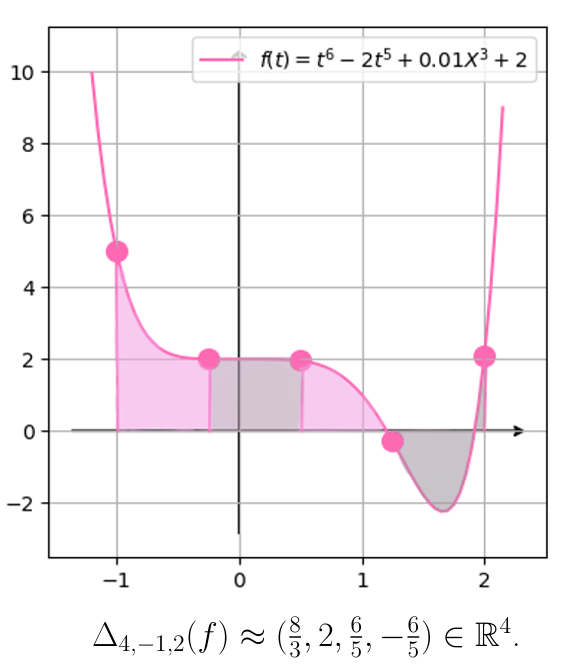
\includegraphics[scale=1]{1En_2} 
		\caption{Ejemplo con $n=4$, $a=-1$, $b=2$ y
		$f(t)= t^{6}-2t^{5}+0.01t^{3}+2$}
\end{marginfigure}


\begin{defi}
(\textbf{Operador de discretización $\Delta_{n,a,b}$})
Dados dos números reales $a<b$, se divide
regularmente al intervalo $[a,b]$ en 
$n$ subintervalos de longitud $h=\frac{b-a}{n}$,
es decir, consideramos la partición


\begin{equation}
\label{eq1: 2En}
\cali{P}_{n}= \{ t_{j} \}_{j=0}^{n}, 
\hspace{0.4cm} \text{con} \hspace{0.2cm}
t_{j}=j\frac{b-a}{n}+a \hspace{0.4cm} \text{para}\hspace{0.4cm}
 0 \leq j \leq n.
\end{equation}
Definimos entonces al operador $\Delta_{n,a,b}$ 
de $\cali{C}[a,b]$ en $\mathbb{R}^{n}$ como
\begin{center}
$\Delta_{n,a,b}(f)= \frac{1}{h} (u_{n,j}(f))_{j=1}^{n},$ \hspace{0.3cm}
$f \in \cali{C}[a,b]$,
\end{center}
donde, para toda $1 \leq j \leq n$,
\begin{center}
$u_{n,j}:= \integ{t_{j-1}}{t_{j}}{f(t)dt}$.
\end{center}
\end{defi}



\noindent
Demostremos que, si escogemos
\begin{itemize}
\item para $0 \leq k \leq n-1$ funciones polinomiales
$g_{k}(t) \in \IR[t]$
\begin{equation}
\label{eq10: 3Nov}
g_{k}(t)= \suma{i=0}{k}{c_{k,i}t^{i}},
\hspace{0.2cm} c_{k, k} >0,
\end{equation}
de grado $k$ y coeficiente principal 
$c_{k,k}$ positivo, 

\item cualquier intervalo $[a,b]$ que partimos 
uniformemente con la malla de $n+1$ puntos
$\cali{P}_{n}= \{ t_{j} \}_{j=0}^{n}$ 
definida en \eqref{eq1: 2En},

\end{itemize}

y si definimos, para toda $0\leq k \leq  n-1$
al vector $u_{k}$ en función de $g_{k}$ como 
\begin{equation}
\label{eq1: 3Nov}
u_{k}:= \Delta_{n,a,b}(g_{k})
= \left( \frac{1}{h} 
\integ{t_{j-1}}{t_{j}}{g_{k}(t)dt} \right)_{j=1}^{n} , 
\end{equation}
entonces los primeros $i$ vectores
de la forma \eqref{eq1: 3Nov}
generan a los espacios $W_{n,i}$
definidos antes en 
\ref{def: espacis Wni},
son linealmente independientes y,
después de ortonormalizarse con 
el proceso de G-S,
obtenemos a los elementos de la base $\cali{L}^{n}$.

Comencemos demostrando la independencia lineal
de los $n$ vectores \eqref{eq1: 3Nov}. Al igual que para
la demostración de la proposición análoga 
\ref{Teorema1},
la prueba de este hecho se basa en el Teorema
fundamental del álgebra.

\begin{prop}
\label{prop: los uk forman una base de Rn}
Sea $n \in \IN$. El 
subconjunto $\{u_{k} : \hspace{0.1cm} 0 \leq k \leq n-1 \}$
de $\IR^{n}$ , con
$u_{k}$ los $n$ vectores definidos en 
\eqref{eq1: 3Nov},
es linealmente independiente.
\end{prop}
\noindent
\textbf{Demostración.}
Supongamos, por el contrario, 
que existen números reales $a_{k}$, con $0 \leq k \leq n-1$,
no todos cero tales que se tenga la siguiente igualdad en $\IR^{n}$:
\begin{equation}
\label{eq8: 3Nov}
\suma{k=0}{n-1}{a_{k}u_{k}}=0.
\end{equation}
Desglosando
la igualdad \eqref{eq8: 3Nov} 
entrada a entrada, descomponemos
a esta en el siguiente sistema de $n$ ecuaciones en $\IR$:
\[
\suma{k=0}{n-1}{ \frac{a_{k}}{h} \int_{t_{j-1}}^{t_{j}}g_{k}(t)\ dt} = 0,
\hspace{0.2cm} 1 \leq j \leq n.
\]
Multiplicando este sistema por $h$, llegamos a las
$n$ igualdades
\begin{equation}
\label{eq2: 2En}
\suma{k=0}{n-1}{a_{k} \int_{t_{j-1}}^{t_{j}}g_{k}(t)\ dt} = 0,
\hspace{0.2cm} 1 \leq j \leq n.
\end{equation}
Por la linealidad de la integral, el sistema \eqref{eq2: 2En}
se reescribe como
\begin{equation}
\label{eq9: 3Nov}
\int_{t_{j-1}}^{t_{j}}p(t)\ dt =0,
\hspace{0.2cm} 1 \leq j \leq n,
\end{equation}


\noindent donde $p$ es el polinomio 
\begin{equation}
\label{eq3: 2En}
p(t):=\suma{k=0}{n-1}{a_{k}g_{k}(t)}. 
\end{equation}
Como todos los polinomios $g_{i}$ son,
por hipótesis, de 
grado menor a $n$ y linealmente independientes
(en el espacio $\IR[t]$),
y se ha supuesto que no
todos los
coeficientes $a_{i}$ son cero, el polinomio
$p$ definido en \eqref{eq3: 2En} es no cero y de grado
menor a $n$. \\

Según el sistema \eqref{eq9: 3Nov}, en cada uno
de los intervalos
\[
I_{j}:=[t_{j-1}, t_{j}], \hspace{0.2cm} 1 \leq j \leq n,
\]

\noindent la función polinomial $p$, continua en todos ellos, 
integra cero. \\

Ahora bien, si en $I_{j}$ la función $p$ fuese siempre
positiva, la integral de esta sería positiva; si fuese
siempre negativa, la integral también. Existen entonces
puntos $a_{j}$ y $ b_{j}$ en $I_{j}$ tales que
\[
p(a_{j})<0 \hspace{0.2cm} \text{y}
\hspace{0.2cm} p(b_{j})>0.
\]

\noindent Aplicando el teorema del valor intermedio
(c.f. \cite{spivak} p. 109)  
deducimos la existencia de un 
$r_{j}$ entre $a_{j}$ y 
$b_{j}$ (y que entonces será punto
interior de $I_{j}$) tal que $p(r_{j})=0$;
así, para cada $1 \leq j \leq n$,
hemos
encontrado una raíz $r_{j}$ de $p$ en 
el interior de $I_{j}$;
por ser ajenos los interiores de los intervalos $I_{j}$,
estamos seguros de que las $n$ raíces $r_{j}$ son distintas
entre sí.
Llegamos así
a que el polinomio no cero $p$, cuyo grado es a lo más $n-1$,
tiene al menos $n$ raíces distintas; esto
contradice la proposición \ref{prop: cita TFA}.
\QEDB
\vspace{0.2cm}

\begin{prop}
\label{prop: uk son discretizaciones pol...}
Sean $n \in \IN$. Para toda $0 \leq k\leq n-1$, si
$g_{k} \in \IR[t]$ es como en \eqref{eq10: 3Nov}
y $u_{k} \in \IR^{n}$ como en
\eqref{eq1: 3Nov}, entonces
$u_{k}$ es la discretización en una malla uniforme
de $n$ puntos de un polinomio de grado $k$
y coeficiente principal positivo. En particular,
$u_{k} \in W_{n,k}$.
\end{prop}
\noindent
\textbf{Demostración.}
La $j-$ésima entrada del vector $u_{k}$
(con $1 \leq j \leq n$)
es, según la igualdad \eqref{eq1: 3Nov},

\begin{align} 
\frac{1}{h} \int_{t_{j-1}}^{t_{j}}{g_{k}(t)} \,dt = &
\frac{1}{h} \int_{t_{j-1}}^{t_{j}}{\suma{i=0}{k}{c_{k,i}t^{i}}} \,dt 
\nonumber \\
= & \frac{1}{h} \suma{i=0}{k}{\int_{t_{j-1}}^{t_{j}}{c_{k,i}t^{i}} \, dt}
\nonumber \\
= & \frac{1}{h} \suma{i=0}{k}{
\frac{c_{k,i}}{i+1}t^{i+1} | ^{t=t_{j}}_{t=t_{j-1}}
} 
\nonumber \\
= & \frac{1}{h} \suma{i=0}{k}{
\frac{c_{k,i}}{i+1}t^{i+1} | ^{t=t_{j-1}+\frac{b-a}{n}}_{t=t_{j-1}}} 
\nonumber \\
= & 
\frac{1}{h} \suma{i=0}{k}{
\frac{c_{k,i}}{i+1} \left( t_{j-1}+ \frac{b-a}{n} \right)^{i+1}}-
\frac{1}{h} \suma{i=0}{k}{
\frac{c_{k,i}}{i+1} t_{j-1}^{i+1}}; \nonumber\\
\end{align}
esta última expresión, en principio, es un polinomio
de grado a lo más $k+1$,
que denotaremos por $q_{k}$, evaluado en $t_{j-1}$,
y que está dado por la expresión
\begin{equation} \label{eq2: 5Nov}
q_{k}(t)= \frac{1}{h} \suma{i=0}{k}{
\frac{c_{k,i}}{i+1} \left(t+ \frac{b-a}{n} \right)^{i+1}}-
\frac{1}{h} \suma{i=0}{k}{
\frac{c_{k,i}}{i+1} t^{i+1}}.
\end{equation}

\begin{itemize}
\item Note que las potencias de orden $k+1$ del argumento
$t$ en la expresión \eqref{eq2: 5Nov}
se dan
cuando en la primera y segunda suma el índice $i$
vale $k$; 
tal parte de la suma es 
\begin{equation}
\label{eq1: 5Nov}
\frac{1}{h} \frac{c_{k,k}}{k+1} \left(t+\frac{b-a}{n} \right)^{k+1}-
\frac{1}{h} \frac{c_{k,k}}{k+1} t^{k+1}=
\frac{1}{h} \frac{c_{k,k}}{k+1} t^{k+1}-\frac{1}{h} \frac{c_{k,k}}{k+1} t^{k+1}+ (*)=(*),
\end{equation} 
donde $(*)$ denota un sumando que no contiene potencias de orden
$k+1$ de $t$ (y que, por lo tanto, no interesa para conocer
el coeficiente de $t^{k+1}$).
Así, según \eqref{eq1: 5Nov}, el grado
de $q_{k}$ es a lo más $k$.
\item Busquemos ahora el coeficiente de $q_{k}$ asociado a la
potencia $k$; aparece en
el lado derecho de \eqref{eq2: 5Nov} la potencia $k$
de $t$ cuando en el primer sumando $i=k, k-1$
y también cuando en el segundo sumando $i=k-1$;
así, el coeficiente buscado es
\begin{equation}
\label{eq3: 5Nov}
\frac{1}{h} \frac{c_{k,k}}{k+1}(k+1)\frac{b-a}{n} 
+\frac{1}{h} \frac{c_{k,k-1}}{k}-
\frac{1}{h} \frac{c_{k,k-1}}{k} = 
\frac{c_{k,k}(b-a)}{hn}.
\end{equation}
Puesto que, por hipótesis (c.f. 
condición \eqref{eq10: 3Nov})
el número $c_{k,k}$ es positivo, tenemos que 
el coeficiente principal \ref{eq3: 5Nov}
de $q_{k}$ es positivo.
\end{itemize}


Según todo lo anterior, $u_{k}$
es el polinomio discreto obtenido al evaluar
al polinomio $q_{k}$ (cuyo grado es $k$ y tiene
coeficiente principal \eqref{eq3: 5Nov},
de hecho, es positivo)
en la malla uniforme 
$\cali{P}_{n}=\{t_{j}\}_{j=0}^{n-1}$.
De esto y el teorema 
\ref{cor: propiedades importantes de espacios Wi}
se deduce la pertenencia de $u_{k}$ al espacio $W_{n,k}$.
\QEDB
\vspace{0.2cm}

Recapitulemos; hemos demostrado que 
el subconjunto
\begin{equation}
\label{eq4: 2En}
\{u_{k}: \hspace{0.2cm} 0\leq k \leq n-1 \}
\end{equation}
de $\IR^{n}$
\begin{itemize}
\item es linealmente independiente 
(c.f. proposición \ref{prop: los uk forman una base de Rn}), y que,
\item para toda $0\leq k \leq n-1$, $u_{k}$
es la discretización en una malla uniforme
de $n$ puntos de un polinomio de grado $k$
y coeficiente principal positivo
(c.f. proposición \ref{prop: uk son discretizaciones pol...}),
luego, 
$u_{k} \in W_{n, k}$ (c.f. teorema 
\ref{cor: propiedades importantes de espacios Wi});
\end{itemize}
así, \eqref{eq4: 2En} es una colección de
polinomios que satisface las condiciones pedidas  
en la subsección
\ref{Generalización que involucra a la discretización Omega n}.
Concluimos, según lo demostrado en esa subsección, 
que el resultado de ortonormalizar la 
base $\{u_{k}\}_{k=0}^{n-1}$ de $\IR^{n}$
(construida, recuerde, a partir del operador de 
discretización $\Delta_{n, a, b}$)
es nuestra base de Legendre
discreta definida en 
\ref{def: base de Legendre discreta}.

\begin{figure}[H]
	\sidecaption{
	Según lo demostrado, podemos discretizar a los
	polinomios 
	$f_{k}$, $0 \leq k \leq n-1$ con el operador $\Delta_{n,-1,1}$
	para obtener una colección de vectores
	$\{u_{k} : \hspace{0.1cm} 0 \leq k \leq n-1\}$
	que, después de ortonormalizarse con el algoritmo de
	Gram-Schmidt, de lugar a la base $\cali{L}^{n}$.
	En la figura se ilustra este proceso para cuando $n=4$.
	\label{fig: definicion original legendre discreto}
	}
	\centering
	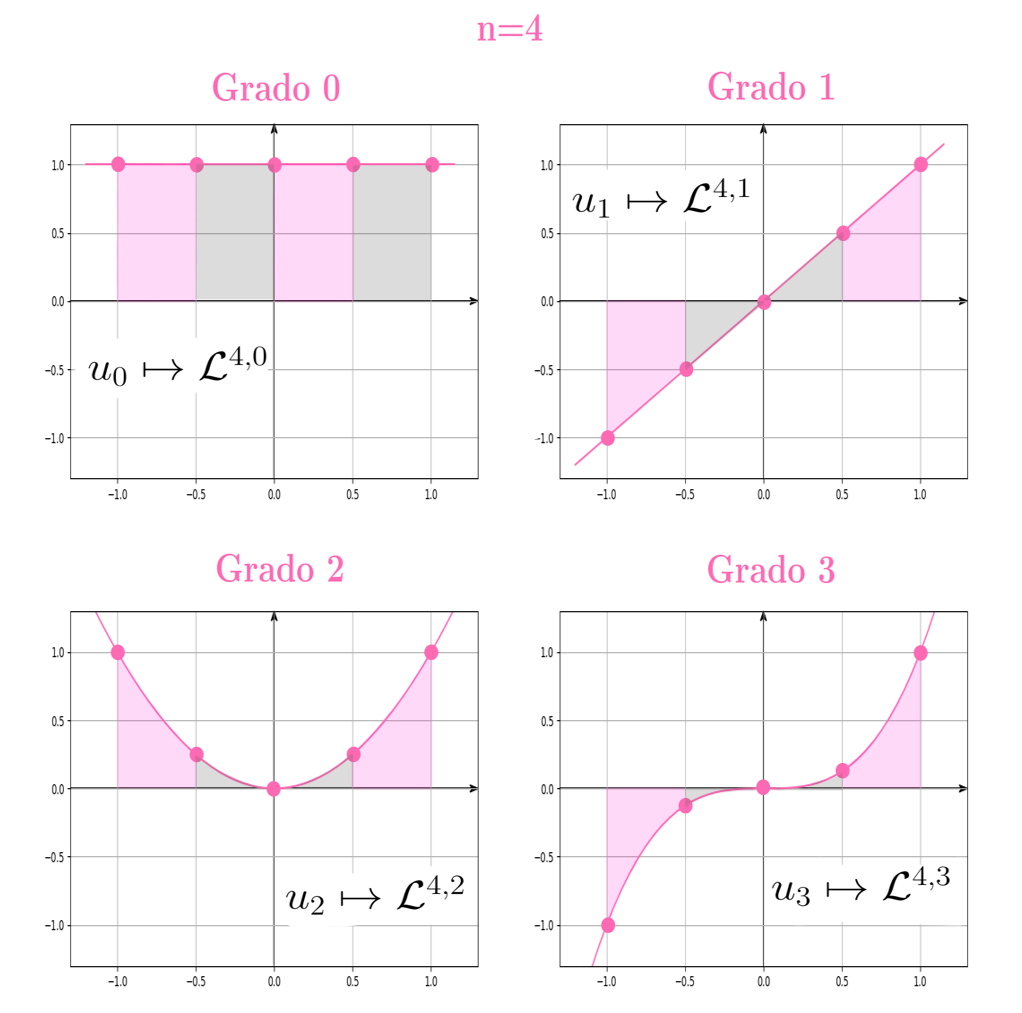
\includegraphics[scale=0.6]{5Dic_1} 
\end{figure}	

        
\begin{figure}[H]
	\sidecaption{
	Según la teoría
	desarrollada, 
	fijada una dimensión $n$ podemos
	cambiar tanto la malla uniforme como el método 
	de discretización; después
	de ortonormalizar, salvo por cambios de signo,
	llegaremos a la
	base $\cali{L}^{n}$. 
	Es el coeficiente principal del polinomio
	que se discretizará
	el que determina
	el signo correcto. Para el ejemplo mostrado
	en la imagen (donde se ha fijado $n=4$), se
	han considerado a los polinomios
	$h_{0}(t)=0.3$, $h_{1}(t)=-0.4t+1$,
	$h_{2}(t)=0.5t^{2}-0.5t$ y $h_{3}(t)=-t^{3}+2t^{2}+t-2$.
	Como se destaca, los polinomios con coeficiente principal
	negativo 
	dan lugar a los respectivos polinomios de Legendre
	discretos con signo negativo.  
	\label{fig: aahm}}
	\centering
	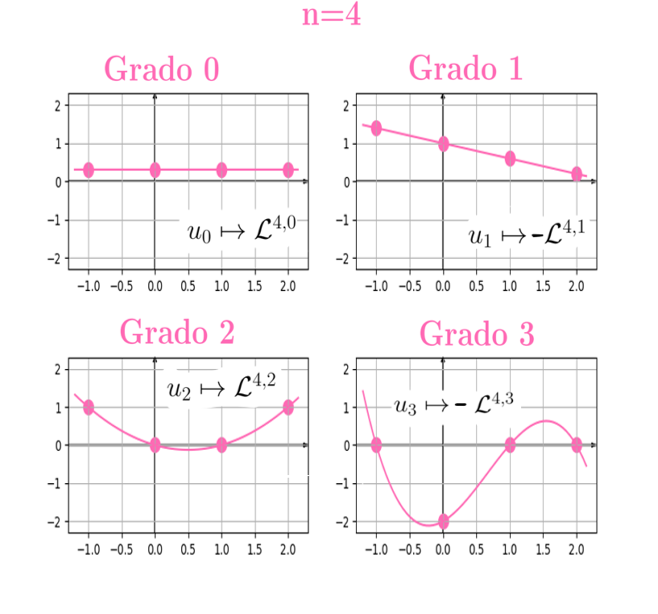
\includegraphics[scale=0.5]{5Dic_2} 
\end{figure}	